\documentclass[a4paper,12pt]{scrartcl}


% deutsche Silbentrennung
\usepackage[english]{babel}
\let\latinencoding\relax
% eigene, zusätzliche Silbentrennung
\usepackage{hyphsubst} %Manuelle Sil\-ben\-tren\-nung
\usepackage[utf8]{inputenc}
\usepackage{amsmath}
\usepackage{amsfonts}
\usepackage{amssymb}
\usepackage{verbatim} 
\usepackage{hyperref}
 
  
% Seitenränder
\usepackage{geometry}
\geometry{a4paper, top= 25mm, bottom=20mm, left = 25mm, right = 25mm, footskip= 1cm}
\setlength\parindent{0pt}

\usepackage{graphicx}
%\includegraphics[width=0.5\textwidth]{images/img1} oder scale=1

% Zeilenabstand (Unterscheidet sich evtl von den Standard 1.5)
\usepackage{setspace}
\linespread{1.5}

\usepackage{fontspec}
%\setmainfont{Times New Roman}
\usepackage{booktabs}
\usepackage{multirow}
\usepackage{wrapfig}
%\usepackage{caption}

\usepackage{cancel}
\usepackage{csquotes}

\usepackage{colortbl}
\usepackage{xcolor}
%\usepackage{hyperref}
%\usepackage[all]{hypcap}
\usepackage{float}

\usepackage{pdfpages}
\usepackage[headsepline]{scrpage2}
\pagestyle{scrheadings}
\clearscrheadfoot

\ofoot{\pagemark}
\ohead{\normalfont \headmark}

%bibliography
\usepackage[natbib,style=alphabetic,minnames=2,maxnames=2,uniquelist=false,backend=biber]{biblatex}
\bibliography{bibliography}
\setlength{\bibitemsep}{1.5em}  

\automark{section}
\newcommand{\gr}{\grqq{}}
\newcommand{\gl}{\glqq}
\newcommand{\vs}{\vspace{3pt}}
\newcommand{\red}{{ \color{red} Quelle}} 
\newcommand{\LL}{\ensuremath{\mathcal{L}}}

\newcommand{\N}{\mathbb{N}}
\newcommand{\Z}{\mathbb{Z}}
\newcommand{\Q}{\mathbb{Q}}
\newcommand{\R}{\mathbb{R}}
%\newcommand{\C}{\mathbb{C}}
\newcommand{\F}{\mathbb{F}}

\renewcaptionname{english}{\figurename}{\small{Fig.}}
\renewcaptionname{english}{\tablename}{\small{Tab.}}
\newcommand{\norm}[1]{\left\| #1 \right\|}

% Zeilenabstand (Unterscheidet sich evtl von den Standard 1.5)
\usepackage{setspace}
\linespread{1.5}

\usepackage{fontspec}
%\setmainfont{Times New Roman}
\usepackage{booktabs}
\usepackage{multirow}
\usepackage{wrapfig}
%\usepackage{caption}

\usepackage{cancel}

\usepackage{colortbl}
\usepackage{xcolor}
%\usepackage{hyperref}
%\usepackage[all]{hypcap}
\usepackage{float}

%\usepackage{rotating}
%\newcommand\tabrotate[1]{\begin{turn}{45}\rlap{#1}\end{turn}}

\usepackage{pdfpages}
\usepackage[headsepline]{scrpage2}
\pagestyle{scrheadings}
\clearscrheadfoot

\ofoot{\pagemark}
\ohead{\normalfont \headmark}
%\cfoot{\normalfont Mathematik \& Informatik}
\automark{section}
\newcommand{\gr}{\grqq{}}
\newcommand{\gl}{\glqq}
\newcommand{\vs}{\vspace{3pt}}
\newcommand{\red}{{ \color{red} Quelle}} 

\renewcaptionname{english}{\figurename}{\small{Fig.}}
\renewcaptionname{english}{\tablename}{\small{Tab.}}
\begin{document}
	
	
\begin{singlespace}
\begin{titlepage}
	\begin{center}
		
		
\includegraphics[scale=0.6]{wwu}
		
		\large{\textbf{\textsf{Faculty of Mathematics and Computer Science}}\\ 
			Summer Semester 2019} \\
		\vspace{20mm}
        \rule{.8\linewidth}{1pt}\\
        \vspace{3mm}
		\LARGE\textbf{\textsf{Behavioral Context Recognition In-The-Wild from Mobile Sensors}}\\
		%\rule{.2\linewidth}{.5pt}\\
		\rule{.8\linewidth}{1pt}\\

		\vfill
	\end{center}
\begin{flushright}
	\flushright

		\begin{large}
	\singlespacing 		
		\begin{tabular}{rl}

			Authors: & Daniel Beckmann \\ & Joschka Strüber \\& Tony Prange \\& Thomas Poschadel \\
			 \midrule
			Lecturers: & Prof. Jiang Xiaoyu \\
					& Sören Klemm \\
			Class:& Pattern Recognition and Machine Learning \\
			Submission deadline: & 13.09.2019

		\end{tabular}
		\end{large}	
\end{flushright}
	
\flushleft
\end{titlepage}

\newpage  \tableofcontents \thispagestyle{empty} \vspace{15mm}
\begin{center}
	\parbox{.8\linewidth}{\begin{small}
			{Beim Nachweis von Zitaten und Literatur wenden wie die von Unisa 
				vorgeschriebene Harvard-Methode an und folge dabei den Regeln 
				in: 
				
				Christof Sauer (Hg.) 2004. 
				Form bewahren: Handbuch zur 
				Harvard-Methode. 
				(GBFE-Studienbrief 5). Lage: Gesellschaft für 
				Bildung und Forschung in Europa e.V. 1. Auflage.} \\
			
			\end{small}}
\end{center}

\end{singlespace}
\newpage
\setcounter{page}{1}

\section*{Abstract}

strg F deepL

\section{Introduction}
A large amount of data is available through the networking of our digital devices, which shape our everyday lives. The use of such data and the associated information is a core element of today's digital society. Programs that can use such data to generate as much information as possible play an important role at improving our daily lives. Those programs are of great interest, not only at the level of contextual advertising, but also in improving our medical care and our behaviors. For example, many people are already optimizing their personal lifestyles with the help of digital devices like smartphone and fitness trackers. Another application is the establishment of a healthy sleep rhythm by the recognition of sleep phases. 

In the context of health care, this technology is of particular interest because on the one hand it can be used preventive. For example, people can be informed about their personal habits and sensitized to their personal risks which arise with their specific lifestyle in order to lead them to a healthier lifestyle, which in turn can be supported by technology again. On the other hand there is the medical perspective, where it is possible to check how healthy a person lives in order to combat diseases more effectively. In conclusion, deriving activities from various sensor data is important for many companies or health organizations, but also for the end user.

The present report was written during a practical course in computer science in the lecture Pattern Recognition, led by Prof. Dr. Xiaoyi Jiang and Sören Klemm, with the topic \gl Behavioral context recognition in-the-wild from mobile sensors\gr (Quelle). The aim of the project was to perform multi-label classification on the basis of the Extrasensory data set. Essentially, collected sensor data should be assigned to activities, in an additional task the users should be recognized by their data. 

The particular challenge of the project was that on the one hand the methodology was not specified and on the other hand multi-label classification was to be carried out with a data set containing many missing labels. 

\section{Introduction of The ExtraSensory Dataset}

The ExtraSensory data set was collected in 2015 and 2016 by Yonatan Vaizman and Katherine Ellis under the supervision of Professor Gert Lanckriet. It is based on sensor data from smartphones and smartwatches produced by 60 participants in intervals of one minute. In contrast to many other data sets, the data was generated by normal everyday devices using multiple sensors were in parallel. Furthermore, the participants behavior was not scripted like in many other case studies and they were allowed to behave in an natural way. The sensors included an accelerometer, gyroscope, location and audio sensor and were used by almost everyone in most of the recordings. Additionally some participants used smart watches or fitness tracker which provided an addition watch accelerometer.

The assignment of the data points to activities was mostly done by the users themselves, who had the option to use predefined labels or create their own. In a preprocessing step these label were reduced to a set of 51 labels by combining similar label. The result were 377,346 data points, which were described with one or more of the 51 final labels. The label represent various information about the location, the context and the activity of a user. some examples are 'in class', 'singing', 'stairs (going up)', 'stairs (going down)', 'with friends' or 'talking'.

This means that for each data point a label vector of length 51 exists. Each entry can contain the values true, false or NaN, where NaN represents missing information on this label. The following examination of the data points shows that many labels remained unobserved in each data point:

\begin{figure}[H]
	\begin{center}
		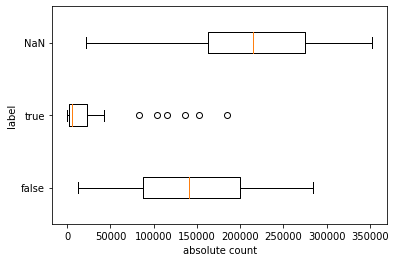
\includegraphics[scale=.8]{images/boxplot_label.png}
		\caption{A box-plot showing the distribution of the absolute count of a given value (false, true or NaN) over the different labels. The yellow line represents the median, the rectangle the 25\% percentile, the line the 75\% percentile and the dotes are outliers.}
		\label{abb:boxplot_label}
	\end{center}		
\end{figure}	

Figure \ref{abb:boxplot_label} visualizes the distribution for each label and a specific value (false, ture or NaN) as a box-plot diagram. Looking at the median for NaN, it can be seen that for most labels the majority of data points do not contain a value - which increases the difficulty of classification. This means that for many labels there is a large number of data points that do not contain any information about the label.

Furthermore, it can be seen that the median labels with the value true is just 5,153 and that only very few labels at all are labeled as true for more than 10\% of the data points. So there are many label classes which contain very few positive representatives. 

\begin{figure}[H]
	\begin{center}
		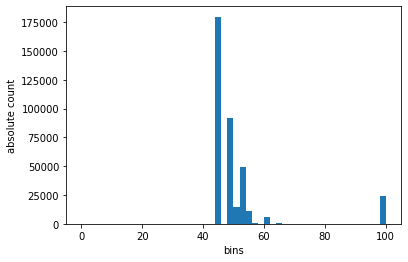
\includegraphics[scale=.8]{images/hist.png}
		\caption{Histogram of absolute counts of percentage of NaN values for each data point. The data is distributed into 50 bins. Each bin has the size of 2 \% of the labels.}
		\label{abb:histogramm_data}
	\end{center}		
\end{figure}

Finally, it can be seen that in all data points at least 44\% of the 51 labels are not evaluated. Thus, there are no data points that make statements about all labels at the same time.

\section{Random Forests}

\section{Gradient Boosting}

\subsection{What is Gradient Boosting}

\subsection{Use of Gradient Boosting}

\subsection{eigene Variationen}
-> Hyperparametern
-> Geschwindigkeit (GPU)


\section{Vorstellung Results}
-> Metric

\section{Bewertung der Results}

\section{classification of users}




\newpage
\section{Literaturverzeichnis}

\hangindent+30pt \hangafter=1
\textsc{Drüke-Noe, C.} 2014. \textit{Aufgabenkultur in Klassenarbeiten im Fach Mathematik – Empirische Untersuchungen in neunten und zehnten Klassen}. Wiesbaden:
Springer Spektrum.









\newpage
\ohead{\normalfont Eigenständigkeitserklärung}
\addcontentsline{toc}{section}{Eigenständigkeitserklärung} 
\vspace*{1cm}
\begin{center}
	\Large \textbf{Anti-Plagiatserklärung}\\
	
	\large \textbf{Erklärung des Studierenden}
\end{center}

\normalsize
\vspace{25mm}
Hiermit versichere ich, dass ich die vorliegende Hausarbeit mit dem Namen \glqq {Umsetzung der Kouninschen Klassenführungsdimension \gl Valenz und Herausforderung\gr{} in meinem beruflichen Handeln\grqq{} selbstständig verfasst habe, und dass ich keine anderen Quellen und Hilfsmittel als die angegebenen benutzt habe und dass die Stellen der Arbeit, die anderen Werken – auch elektronischen Medien – dem Wortlaut oder Sinn nach entnommen wurden, auf jeden Fall unter Angabe der Quelle als Entlehnung kenntlich gemacht worden sind.\\
	
	
	
	
	\begin{center}
		\rule{6cm}{.5pt} \hspace{3cm} \rule{6cm}{.5pt}
	\end{center}	
	\vspace{-5mm}
	\hspace*{25mm} Ort, Datum	\hspace{70mm} Tony Prange


\end{document}